% vim:ft=tex

\section{Distance Database}

\subsection{Algorithm}

If we computed the distance between all cities in Europe, it would take a very
long time and file the hard drive consequently.
To reduce the effort was decided to group each postcode by its region (most of the
time represented by the two first digits). Then we compute the distance ``as the
crow flies'' and by road between each of these regions and store them into the database.

When requesting the distance between two postcode, we process as such:
\begin{enumerate}
  \item transform both postcode into coordinates
  \item calculate the distance as the crow flies (named $d_{direct,crow}$)
  \item determine the two 2-digit regions associated
  \item get the distance ``as the crow flies'' ($d_{region,crow}$) and by road
      ($d_{region,road}$) between the two regions from the database
  \item calculate the ratio $ratio = d_{region,road}/d_{region,crow}$
  \item the final distance estimate is $d_{direct,crow} * ratio$
\end{enumerate}

The calculation is summarized by figure~\ref{fig:calc}.
\begin{figure}[H]
\centering
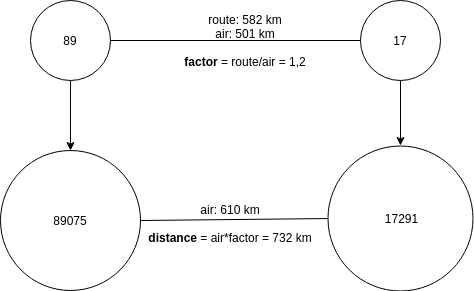
\includegraphics[width=0.7\textwidth]{img/calc}
\captionof{figure}{Theoretical example of distance calculation}\label{fig:calc}
\end{figure}

\subsection{Filling the Database}

\subsubsection{List of 2-digits Regions}

The countries' regions being often indicated as the two first digits of the
postcodes, we can simply create our groups based on that.
However, we must take into account that there are some exceptions; for instance,
Luxembourg prefixes its postcodes with ``LE-''.
Some other countries also introduce non-alphanumerical characters, such as:
spaces, hyphens, dots, \ldots{}

We also restrict this operation to European countries only, we can do that by filtering
postcodes by their coordinates: Europe being found between -11° West and 41° East,
and 35° to 71° North.

\subsubsection{Calculation of Region's Centroid}

To calculate the centroid for each region, we can compute the average coordinates
of all postcodes of that region. However, we will have to use Graphhopper with
these coordinates and Graphhopper can only work when coordinates point to a
road/street/\ldots{}
To test if a coordinate is working for Graphhopper, we simply query it from our
coordinate to an already checked place.

First, we test Graphhopper for the average centroid. If it can't be used, we go
through the closest postalcodes to find one accepted by Graphhopper. Finally, if
we still don't have a good point, we spiral around the average centroid until we
find a good point or we reach 3 degrees radius (3 degrees in longitude is around
245km in Germany). We discard every other regions that fail these three tests.
